\documentclass{article}%
\usepackage[T1]{fontenc}%
\usepackage[utf8]{inputenc}%
\usepackage{lmodern}%
\usepackage{textcomp}%
\usepackage{lastpage}%
\usepackage[head=40pt,margin=0.5in,bottom=0.6in]{geometry}%
\usepackage{graphicx}%
%
\title{\textbf{Pensionados protestan en Bolívar por pago incompleto}}%
\author{El Nacional Web}%
\date{18/09/2018}%
%
\begin{document}%
\normalsize%
\maketitle%
\textbf{URL: }%
http://www.el{-}nacional.com/noticias/protestas/pensionados{-}protestan{-}bolivar{-}por{-}pago{-}incompleto\_252185\newline%
%
\textbf{Periodico: }%
EN, %
ID: %
252185, %
Seccion: %
Protestas\newline%
%
\textbf{Palabras Claves: }%
Bolívar, Denuncia\newline%
%
\textbf{Derecho: }%
2.6, %
Otros Derechos: %
, %
Sub Derechos: %
2.6.1\newline%
%
\textbf{EP: }%
SI\newline%
\newline%
%
\textbf{\textit{Los adultos mayores aseguran que van al banco diariamente porque necesitan, no porque quieren}}%
\newline%
\newline%
%
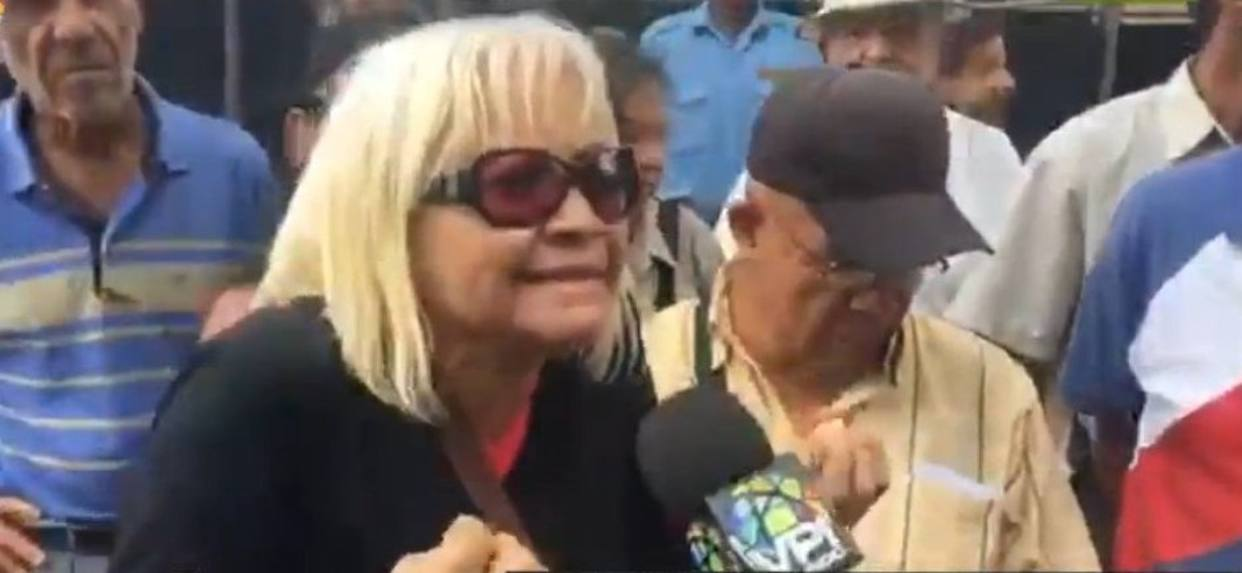
\includegraphics[width=300px]{198.jpg}%
\newline%
%
Pensionados del municipio Caroní,~estado Bolívar,~protestan~este martes por el pago incompleto de sus pensiones.%
\newline%
%
Los adultos mayores denunciaron~retraso en el pago de sus pensiones y aseguraron~que solo les permiten sacar~~BsS~180~en efectivo, por lo que exigen que habiliten más cajas y rechazan el pago dividido de su~pensión.%
\newline%
%
Por otra parte, los pensionados expresaron que las personas duermen en la calle desde el fin de semana para hacer la cola y sacar~efectivo el siguiente día hábil.%
\newline%
%
\end{document}